\section{Configuration of Virtual Machine Cluster}

\subsection{Mirror Configuration}

Fast provisioning and delivery, automation, and ease of scaling are key to today's elastic computing. However, setting up instances one by one, configuring their cumbersome dependencies and environment variables, and installing them by downloading source code and binary packages from the web and configuring them by copy and paste is typical of UNIX mainframe administrators in the 1980s.

Compared to the handbook \cite{li-chao} suggests that using an Ubuntu image and configure them manually, we've built a custom mirror, which already has Hadoop, Spark, and SBT packed up and modified. We referenced the image creation tool provided by Arch Linux on \cite{Arch-box} with the Cloud-init tool and rewrote the compiling script of the Hadoop package on \cite{hadoop-package} to match the \texttt{JAVA\_HOME} lookup process. A system installation script was written to suit the needs of this experiment. This series of configuration files are placed in the submitted files' \texttt{image-buildscript} folder.

Many cloud providers has provided custom image service, so do Huawei Cloud. By utilizing its IMS services \cite{IMS} as figure \ref{fig:ims}, we can now create virtual machines with our pre-built images.

\begin{figure}[ht]
    \centering
    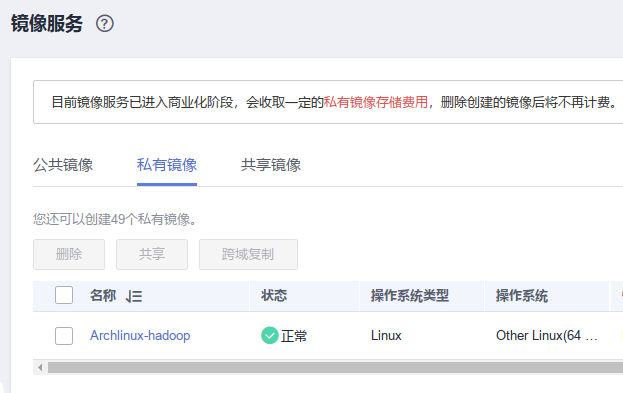
\includegraphics[width=\figurewidth]{figure/hadoop-image.png}
    \caption{Huawei Cloud IMS}
    \label{fig:ims}
\end{figure}

\subsection{Virtual Machine Configuration}

To perform VM configuration as designed in our mirror, adjusting roles while the VM is created, we use Huawei Cloud SDK and its OpenAPI to perform creation. The core part is to utilize OpenStack \texttt{user\_data}. When the \texttt{user\_data} is provided as bash scripts, it will be run at VM creation by cloud-init. The script we created performs Hadoop configuration according to Hadoop Documentation \cite{Hadoop-setup}, worker appointment, and SSH key configuration. This series of configuration scripts and API call Python scripts are placed in the submitted files' \texttt{HuaweiCloud-openAPI} folder.

\subsection{Hadoop Initiation}

By running the commands below: (Our Hadoop instance is installed under \texttt{/usr/lib})

\begin{verbatim}
cd /usr/lib/hadoop
bin/hdfs namenode -format
sbin/start-all.sh   
\end{verbatim}

The Hadoop instance will be set up, and can be viewed via \texttt{http://master:9870} as in figure \ref{fig:DN-info}.

\begin{figure}[ht]
    \centering
    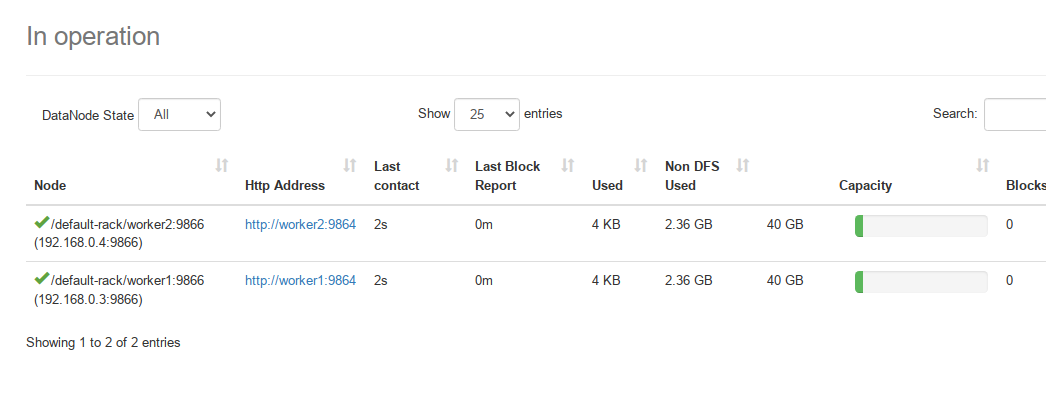
\includegraphics[width=\figurewidth]{figure/configured-hadoop.png}
    \caption{DataNode Information on NameNode}
    \label{fig:DN-info}
\end{figure}